% \iffalse
\let\negmedspace\undefined
\let\negthickspace\undefined
\documentclass[journal,12pt,twocolumn]{IEEEtran}
\usepackage{cite}
\usepackage{amsmath,amssymb,amsfonts,amsthm}
\usepackage{algorithmic}
\usepackage{graphicx}
\usepackage{textcomp}
\usepackage{xcolor}
\usepackage{txfonts}
\usepackage{listings}
\usepackage{enumitem}
\usepackage{mathtools}
\usepackage{gensymb}
\usepackage{comment}
\usepackage[breaklinks=true]{hyperref}
\usepackage{tkz-euclide} 
\usepackage{listings}
\usepackage{gvv}                                        
\def\inputGnumericTable{}                                 
\usepackage[latin1]{inputenc}                                
\usepackage{color}                                            
\usepackage{array}                                            
\usepackage{longtable}                                       
\usepackage{calc}                                             
\usepackage{multirow}                                         
\usepackage{hhline}                                           
\usepackage{ifthen}                                           
\usepackage{lscape}
\usepackage{tabularx}

\newtheorem{theorem}{Theorem}[section]
\newtheorem{problem}{Problem}
\newtheorem{proposition}{Proposition}[section]
\newtheorem{lemma}{Lemma}[section]
\newtheorem{corollary}[theorem]{Corollary}
\newtheorem{example}{Example}[section]
\newtheorem{definition}[problem]{Definition}
\newcommand{\BEQA}{\begin{eqnarray}}
\newcommand{\EEQA}{\end{eqnarray}}
\newcommand{\define}{\stackrel{\triangle}{=}}
\theoremstyle{remark}
\newtheorem{rem}{Remark}
\begin{document}
\bibliographystyle{IEEEtran}
\vspace{3cm}

\title{NCERT-discrete : 10.5.3 - 2}
\author{EE23BTECH11025 - Anantha Krishnan $^{}$% <-this % stops a space
}
\maketitle
\newpage
\bigskip



\section{question}
\vspace{0.5cm}
Find the sums given below:
\begin{enumerate}
    \item[(i)] 7 + $10\dfrac{1}{2}$ + 14 ... + 84
    \item[(ii)] 34 + 32 + 30 ... + 10
    \item[(iii)] -5 + -8 + -11 ... -230

\end{enumerate}

\vspace{0.5cm}
\textbf{Solutions}:
\begin{enumerate}
\item[(i)]   
7 + $10\dfrac{1}{2}$ + 14 ... + 84\\
\vspace{0.2cm}

Let "$S_{k}$" denote the sum of first k terms in a series ,"a" denotes its first term and "d" denotes the common difference.
\begin{align}
{S_k} = \dfrac{k}{2}(2a + (k-1)d)\label{eq:1}
\end{align}
For number of terms , we use
\begin{align}
x(n) = x(0) + nd\label{eq:2}
\end{align}
Where x(n) is the $(n+1)^{th}$ term of the series. Putting the values
\begin{align}  
84 = 7+\dfrac{7n}{2}\\
n=22
\end{align}
\textbf{Calculating $S_n$ for $x_{1(n)}$ }\\
We now use this result for calculating $S_{23}$
\begin{align}
    S_{23} = \dfrac{23}{2}(14+(22)\dfrac{7}{2})
    \end{align}
Solving this yields $S_{23}$ = 1046.5\\\\
We are now required to calculate $X_{1(z)}$ in terms of $u_n$ and $x_{1(n)}$.Where u$_{(n)}$ is the unit step function.
\begin{align}
    x_{1(n)} = u_{(n)}(x_{1(0)}+\dfrac{7n}{2})
    \end{align}
    \begin{figure}[!ht]
    \centering
\graphicspath{ {figs/} }
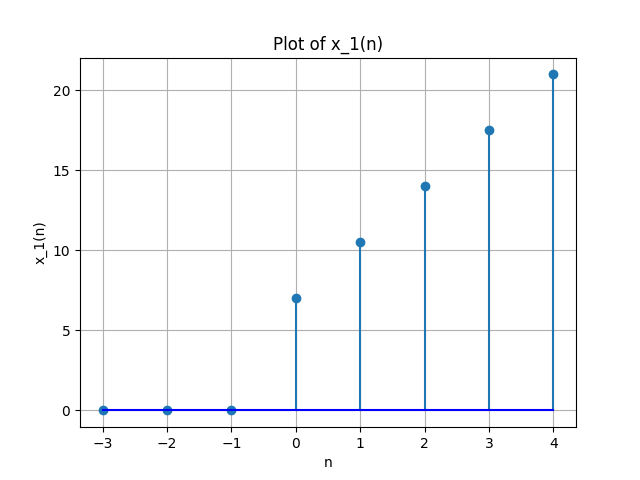
\includegraphics[width=10cm, height=6cm]{graph_1}
\captionsetup{Graph:1 $x_{1(n)}$ vs n }
\end{figure}
\\\\\\\\
\textbf{Z-Transform of $x_{1(n)}$}\\
\vspace{0.2cm}
By the Definition of Z-transform:
\begin{align}
 \sum_{n=-\infty}^{\infty} Z^{-n}x(n) = X(Z)\label{eq:3}
 \end{align}
\\Putting $x_{1(n)}$ in $\eqref{eq:3}$ , we get \\
\begin{align}
     \sum_{n=-\infty}^{\infty}(x_{1(0)} + \dfrac{7n}{2})u_{(n)}Z^{-n} =X_{1(z)}
\end{align}
\begin{align}
\sum_{n=-\infty}^{\infty}(7 + \dfrac{7n}{2})u_{(n)}Z^{-n} =X_{1(z)}
\end{align}
For the \textbf{region of convergence}\\
$X_{1(z)}$ = convergent $\forall$ z $\epsilon$(-\infty,-1)U(1,\infty)
\\

This can be proved from ratio test . \\
We now calculate the sum (Here $(k-1)^{th}$ term is the last term and  $x_{1(0)}$ is the first term).
\begin{align}
   \notag 7(1-z^k)(z^k(1-z))^{-1}+
   \\ \notag(7(z^k-1)z)(2z^k(z-1)^2)^{-1}-\\ (7kz)(2z^{k+1}(z-1))^{-1}=X_{1(z)}
\end{align}
\\
\\
\vspace{0.5cm}
\item[(ii)]
 34 + 32 + 30 ... + 10\\
\vspace{0.2cm}

In this bit \\ a=34 , d=-2
Using equation \eqref{eq:2}
\begin{align}
     10 = 34 -2n\\
     n=12 
     \end{align}
For $x_{2(n)}$
\begin{align}
x_{2(n)} = x_{2(0)} + nd\\
x_{2(n)} = x_{2(0)} -2n
\end{align}

\begin{figure}[!ht]
\centering
  \graphicspath{ {figs/} }
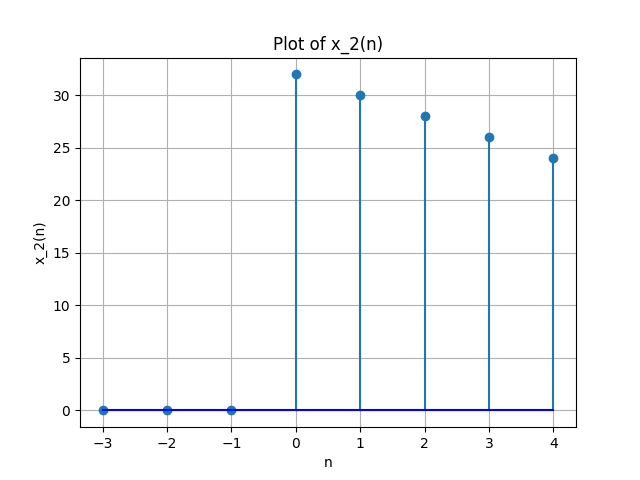
\includegraphics[width=10cm, height=6cm]{graph_2}
\captionsetup{Graph:2 $x_{2(n)}$ vs n }
\label{graph:3}
\end{figure}

\\
\textbf{Z-Transform of $x_{2(n)}$}\\
Using \eqref{eq:3}\\
\begin{align}
\sum_{n=-\infty}^{\infty}(x_{2(0)} -2n)u_{(n)}Z^{-n} =X_{2(z)}
\end{align}
Region of convergence does not change as the nature of the function remains the same as (i)bit\\
For $X_{2(z)}$ , we use the same process as in (i)bit.
\begin{align}
   \notag 32(1-z^k)(z^k(1-z))^{-1}-
   \\ \notag(2(z^k-1)z)(z^k(z-1)^2)^{-1}+\\ (2kz)(z^{k+1}(z-1))^{-1}=X_{2(z)}
\end{align}

\textbf{Calculating $S_n$ of $x_{2(n)}$}\\
For calculating the sum , we use \eqref{eq:1}
\begin{align}
 S_{13} = \dfrac{13}{2}(64+11(-2))\\
 S_{13}= 286.
 \end{align}
 
\vspace{0.5cm}
\item[(iii)]
-5 + -8 + -11 ... -230\\
\vspace{0.2cm}

Here a=-5, d=-3\\
From \eqref{eq:2}
\begin{align}
-230= -5 -3n \\
n=75
\end{align}
For $x_{3(n)}$
\begin{align}
x_{3(n)} = x_3{(0)} + nd\\
x_{3(n)}=x_3{(0)} - 3n
\end{align}

\begin{figure}[!ht]   
\centering
\graphicspath{ {figs/} }
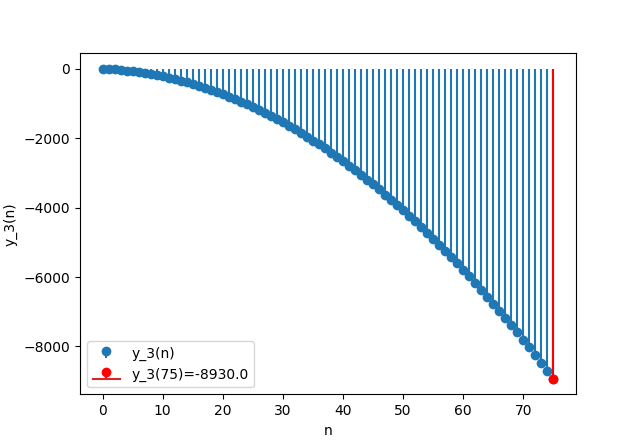
\includegraphics[width=10cm, height=6cm]{graph_3}
\captionsetup{Graph:3 $x_{3(n)}$ vs n }
\label{graph:4}
\end{figure}

\textbf{Z-Transform of $x_{3(n)}$}\\
Putting $x_{3(n)}$ in \eqref{eq:3}\\
\begin{align}
\sum_{n=-\infty}^{\infty}(x_{3(0)} -3n)u_{(n)}Z^{-n} =X_{3(z)}
\end{align}
Region of convergence does not change as the nature of the function remains the same as (i)bit\\
For $X_{3(z)}$ , we use the same process as in (i)bit\\
\begin{align}
   \notag -5(1-z^k)(z^k(1-z))^{-1}-
   \\ \notag(3(z^k-1)z)(z^k(z-1)^2)^{-1}+\\ (3kz)(z^{k+1}(z-1))^{-1}=X_{3(z)}
\end{align}
\textbf{Calculating $S_n$ of $x_{3(n)}$}\\
Using \eqref{eq:1} :\\
\begin{align}
    S_{76}=\dfrac{76}{2}(-10+(76-1)(-3))
   \\S_{76}=-8930
    \end{align}
  
 \newpage
 \begin{center}
\begin{tabular}{ |c|c|c| } 
 \hline
 Parameters & Description & Values    \\ 
 \hline
  $x_{1(n)}$ & Sequence labelled (i) &  $x_{1(0)}$ +3.5n\\
  $x_{2(n)}$ &  Sequence labelled (ii) & $x_{2(0)}$ -2n \\
  $x_{3(n)}$ &  Sequence labelled (iii) & $x_{3(0)}$ -3n \\
   $x_{1(0)}$ & $1^{st}$ term of sequence $x_{1(n)}$ & 7 \\
     $x_{2(0)}$ & $1^{st}$ term of sequence $x_{2(n)}$& 34 \\
     $x_{3(0)}$ & $1^{st}$ term of sequence $x_{3(n)}$ & -5 \\
 $X_{1(z)}$ & Z-Transform of $x_{1(n)}$ & $7(1-z^k)(z^k(1-z))^{-1}+
    (7(z^k-1)z)(2z^k(z-1)^2)^{-1}-(7kz)(2z^{k+1}(z-1))^{-1}$\\
 $X_{2(z)}$ &  Z-Transform of $x_{2(n)}$ & $32(1-z^k)(z^k(1-z))^{-1}-
    (2(z^k-1)z)(z^k(z-1)^2)^{-1}+(2kz)(z^{k+1}(z-1))^{-1}$ \\ 
$X_{3(z)}$ &  Z-Transform of $x_{3(n)}$ & $-5(1-z^k)(z^k(1-z))^{-1}-
    (3(z^k-1)z)(z^k(z-1)^2)^{-1}+(3kz)(z^{k+1}(z-1))^{-1}$ \\
 \hline
\end{tabular}
\centering
\captionsetup{TABLE 1 : PARAMETERS , DESCRIPTIONS AND VALUES }
\end{center}
\end{enumerate}
\end{document}
